% Preamble {{{
\documentclass[11pt,a4paper,titlepage,dvipsnames,cmyk]{scrartcl}
\usepackage[english]{babel}
\typearea{12}
% }}}

% Set indentation and line skip for paragraph {{{
\setlength{\parindent}{0em}
\setlength{\parskip}{1em}
\usepackage[margin=2cm]{geometry}
\addtolength{\textheight}{-1in}
\setlength{\headsep}{.5in}
% }}}

\usepackage{hhline}
\usepackage[table]{xcolor}
\usepackage{mathtools}
\usepackage[T1]{fontenc}

% Headers setup {{{
\usepackage{fancyhdr}
\pagestyle{fancy}
\lhead{Advanced Topics in Programming Languages: Equation List}
\rhead{Josh Felmeden}
\usepackage{hyperref}
% }}}

% Listings {{{
\usepackage[]{listings}
\lstset
{
    breaklines=true,
    tabsize=3,
    showstringspaces=false
}

\definecolor{lstgrey}{rgb}{0.05,0.05,0.05}
\usepackage{listings}
\makeatletter
\lstset{language=[Visual]Basic,
backgroundcolor=\color{lstgrey},
frame=single,
xleftmargin=0.7cm,
frame=tlbr, framesep=0.2cm, framerule=0pt,
basicstyle=\lst@ifdisplaystyle\color{white}\footnotesize\ttfamily\else\color{black}\footnotesize\ttfamily\fi,
captionpos=b,
tabsize=2,
keywordstyle=\color{Magenta}\bfseries,
identifierstyle=\color{Cyan},
stringstyle=\color{Yellow},
commentstyle=\color{Gray}\itshape
}
\makeatother
\renewcommand{\familydefault}{\sfdefault}
\newcommand{\specialcell}[2][c]{%
\begin{tabular}[#1]{@{}c@{}}#2\end{tabular}}
% }}}

% Other packages {{{
\usepackage{graphicx}
\graphicspath{ {./pics/} }
\usepackage{needspace}
\usepackage{tcolorbox}
\usepackage{soul}
\usepackage{babel,dejavu,helvet}
\usepackage{amsmath}
\usepackage{amsfonts}
\usepackage{booktabs}
\usepackage{tcolorbox}
\usepackage[symbol]{footmisc}
\renewcommand{\thefootnote}{\fnsymbol{footnote}}
\renewcommand{\familydefault}{\sfdefault}
\usepackage{enumitem}
\setlist{nolistsep}
% }}}

% tcolorbox {{{
\newtcolorbox{blue}[3][] {
colframe = #2!25,
colback = #2!10,
#1,
}

\newtcolorbox{titlebox}[3][] {
colframe = #2!25,
colback = #2!10,
coltitle = #2!20!black,
title = {#3},
fonttitle=\bfseries
#1,
}
% }}}

% Title {{{
\title{Advanced Topics in Programming Languages: Equation List}
\author{Josh Felmeden}
% }}}

\begin{document}
\maketitle
\tableofcontents
\newpage

\section{Structural Rules}
\subsection{Inversion Lemma}

\begin{tcolorbox} [space to upper,
collower=white,
title={Lemma 1 (Inversion)},
nobeforeafter,
halign lower=flush right, ]
Suppose $\Gamma \vdash e : \tau$.
\begin{enumerate}
\item If $e=\text{plus}(e_1;e_2)$ then it must be that
\begin{itemize}
    \item $\tau = \text{Num}$
    \item $\Gamma \vdash e_1 : \text{ Num}$
    \item $\Gamma \vdash e_2 : \text{ Num}$
\end{itemize}
\end{enumerate}
\end{tcolorbox}

You basically prove this lemma by saying look at the rules there can't be another way. The lemma can also be shown by induction on the typing derivation.

\subsection{Weakening}
Suppose that $x : \sigma \vdash e: \tau$ ($e$ computes a value of type $\tau$ if $x$ is of type $\sigma$). It is fair to say that for any \textbf{fresh variable} $y$ (a variable that doesn't already appear in term $e$), the typing judgement $x: \sigma, y:\rho \vdash e:\tau$ should also hold no matter what type $\rho$ is. Essentially, assuming random free variables that are unused should not influence the type of a program. This is called \textbf{weakening.} We state and prove by induction on the typing derivation that:

\begin{tcolorbox} [space to upper,
collower=white,
title={Lemma 2 (Weakening)},
nobeforeafter,
halign lower=flush right, ]
If $\Gamma \vdash e:  \tau$ and $x$ is fresh then $\Gamma, x : \sigma \vdash e : \tau$
\end{tcolorbox}

\subsection{Substitution}
\begin{tcolorbox} [space to upper,
collower=white,
title={Lemma 3 (Substitution)},
nobeforeafter,
halign lower=flush right, ]
If $\Gamma \vdash e : \tau$ and $\Gamma, x : \tau \vdash u : \sigma$ then $\Gamma \vdash u[e/x] : \sigma$
\end{tcolorbox}

\newpage
\section{Type Safety}

\begin{tcolorbox} [space to upper,
collower=white,
title={Theorem 1 (Type safety)},
nobeforeafter,
halign lower=flush right, ]
\begin{enumerate}
\item (Preservation) If $\vdash e : \tau$ and $e \mapsto e'$ then $\vdash e' : \tau$
\item (Progress) If $\vdash e : \tau$ then either $e$ val or $e \mapsto e'$ for some $e'$
\end{enumerate}
\end{tcolorbox}

\subsection{Preservation}
Preservation is the statement that types are preserved under evaluation. This is a central \textbf{safety} property of type systems: it shows that a step-by-step computation preserves the kind of value that is being computed. We perform this on dynamics.

\begin{tcolorbox} [space to upper,
collower=white,
title={Theorem 2 (Preservation)},
nobeforeafter,
halign lower=flush right, ]
If $\vdash e : \tau$ and $e \mapsto e'$ then $\vdash e' : \tau$

\textit{Proof}. Using $\vdash e : \tau$, prove that $\vdash e' : \tau$ and if proving some rule $b \longmapsto b'$, also prove $\vdash b' : \tau$.
\textit{Example}: By induction on the derivation of $e \mapsto e'$. We show the most diffcult case, namely that of D-Let: Suppose that the reduction $e \mapsto e'$ is of the form
\begin{align*}
\frac{}{\text{let}(e_1;x,e_2) \mapsto e_2 [e_1/x]}\text{D-Let}
\end{align*}

We know that $\vdash \text{let}(e_1;x.e_2) : \tau$. By \textbf{inversion} there must exist $\sigma$ such that $\vdash e_1 : \sigma$ and $x:\sigma \vdash e_2 : \tau$. By the \textbf{substitution lemma}, we obtain $\vdash e_1[e_1/x] : \tau$.
\end{tcolorbox}

\subsection{Progress}
Progress is the statement that if a well-typed program is not done computing (aka: is a value), then there must be a step of computation it may take. We perform this on statics.

\begin{tcolorbox} [space to upper,
collower=white,
title={Lemma 4 (Canonical Forms)},
nobeforeafter,
halign lower=flush right, ]
Suppose $e$ val:
\begin{enumerate}
\item If $\vdash e : \text{Num}$ then $e = \text{num}[n]$ for some $n \in \mathbb{N}$
\item If $\vdash e : \text{Str}$ then $e = \text{str}[s]$ for some $s \in \Sigma^*$
\end{enumerate}
\end{tcolorbox}

\begin{tcolorbox} [space to upper,
collower=white,
title={Theorem 4 (Progress)},
nobeforeafter,
halign lower=flush right, ]
If $\vdash e : \tau$ then either $e$ val or $e \mapsto e'$ for some $e'$

\textit{Proof}. By induction on the derivation of $\vdash e : \tau$. 
\end{tcolorbox}



\newpage
\section{Judgements}
\subsection{Statics}
\begin{center}
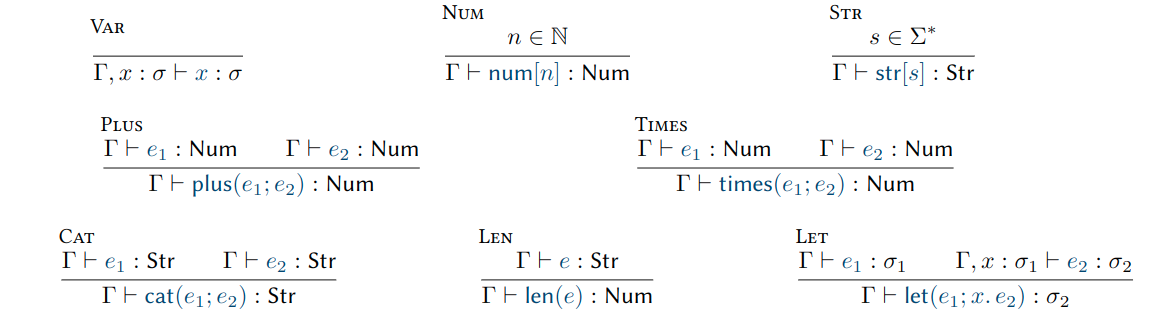
\includegraphics[width=\textwidth]{pics/static-judgement.png}
\end{center}

\subsection{Dynamics}
\begin{center}
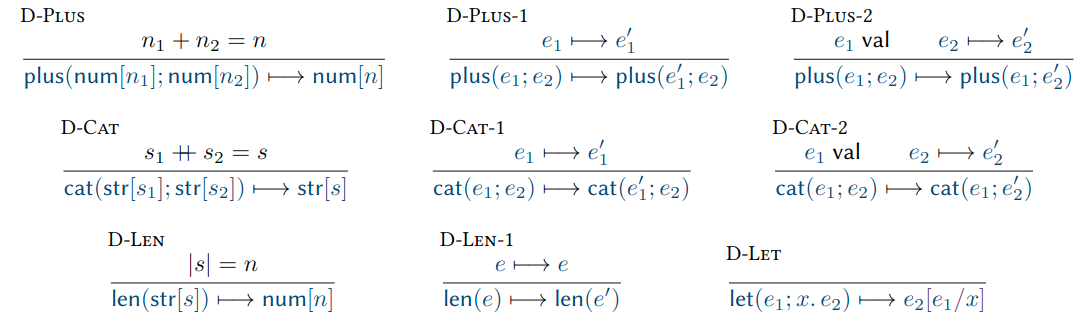
\includegraphics[width=\textwidth]{pics/dynamic-judgement-1.png}
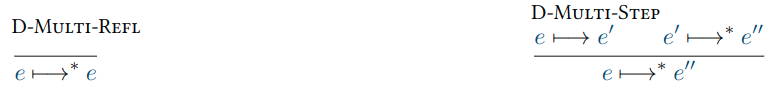
\includegraphics[width=\textwidth]{pics/dynamic-judgement-2.png}
\end{center}

\newpage
\section{Simply-Typed Lambda Calculus}
\subsection{Products}
\subsubsection{Syntax}
\begin{center}
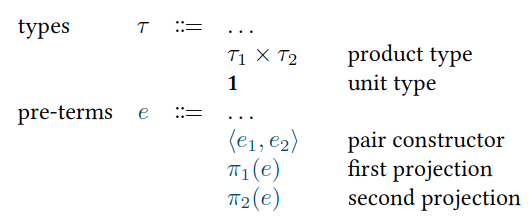
\includegraphics[width=\textwidth/2]{pics/syntax-stlc.png}
\end{center}
\subsubsection{Statics}
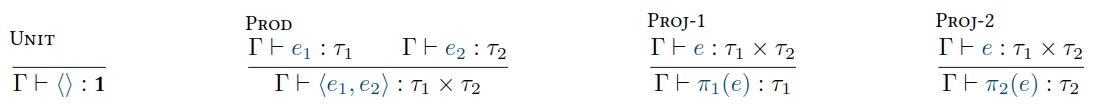
\includegraphics[width=\textwidth]{pics/static-stlc.png}
\subsubsection{Dynamics}
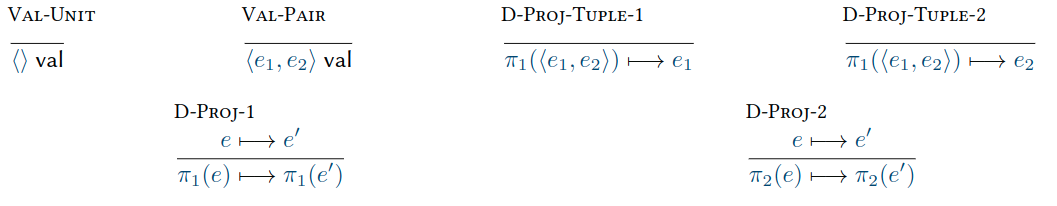
\includegraphics[width=\textwidth]{pics/dynamic-stlc.png}

\subsection{Sums}
\subsubsection{Syntax}
\begin{center}
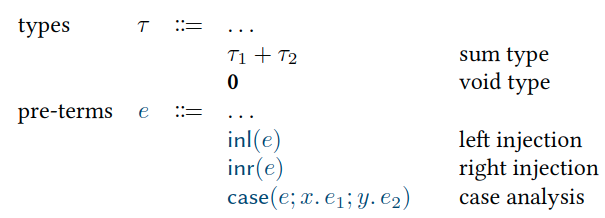
\includegraphics[width=\textwidth/2]{pics/syntax-stlc-sum.png}
\end{center}
\subsubsection{Statics}
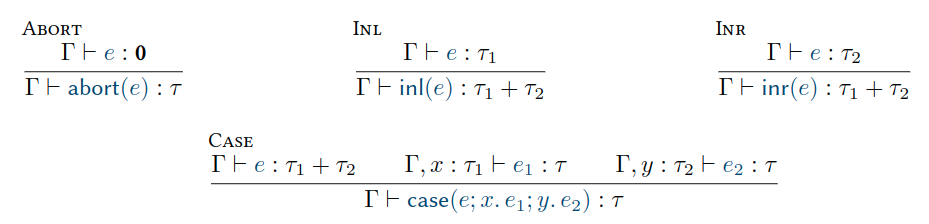
\includegraphics[width=\textwidth]{pics/static-stlc-sum.png}
\subsubsection{Dynamics}
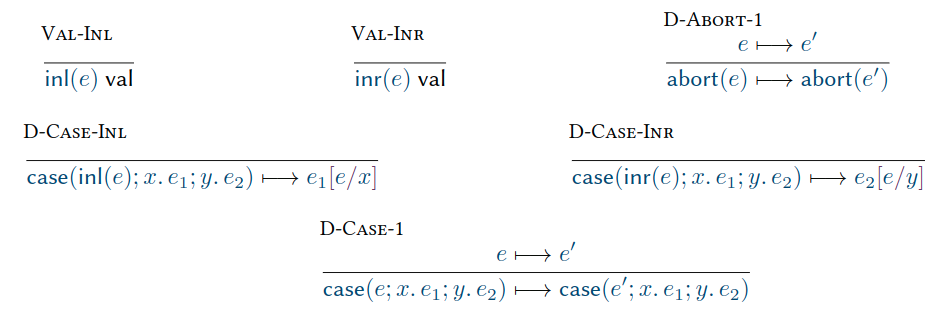
\includegraphics[width=\textwidth]{pics/dynamic-stlc-sum.png}

\subsection{Functions}
\subsubsection{Syntax}
\begin{center}
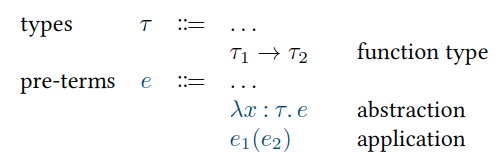
\includegraphics[width=\textwidth/2]{pics/syntax-stlc-func.png}
\end{center}
\subsubsection{Statics}
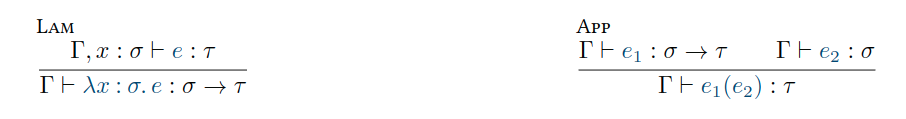
\includegraphics[width=\textwidth]{pics/static-stlc-func.png}
\subsubsection{Dynamics}
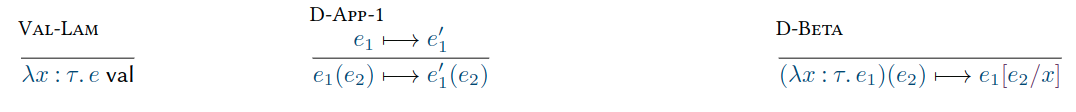
\includegraphics[width=\textwidth]{pics/dynamic-stlc-func.png}

\newpage
\section{Programming Computable Functions (PCF)}
\subsection{Syntax}
\begin{center}
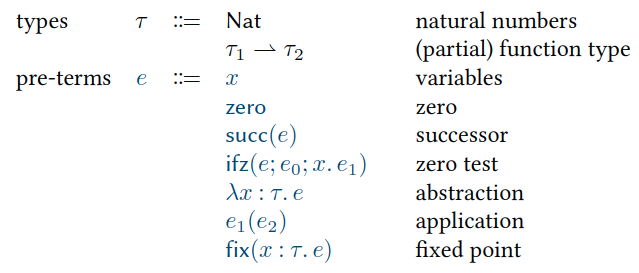
\includegraphics[width=\textwidth/2]{pics/syntax-pcf.png}
\end{center}
\subsection{Statics}
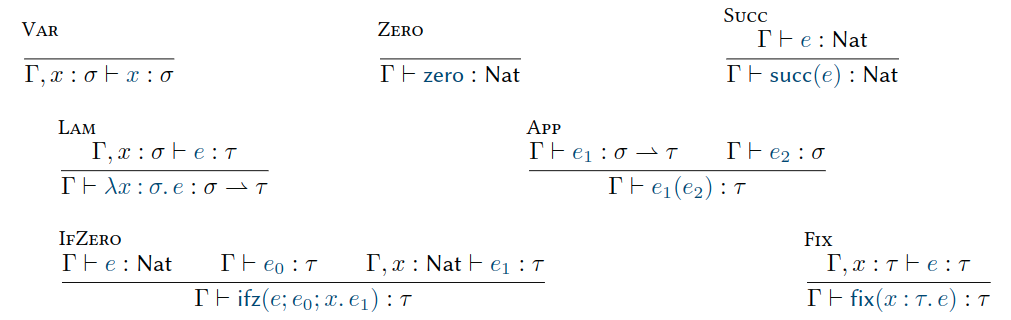
\includegraphics[width=\textwidth]{pics/static-pcf.png}
\subsection{Dynamics}
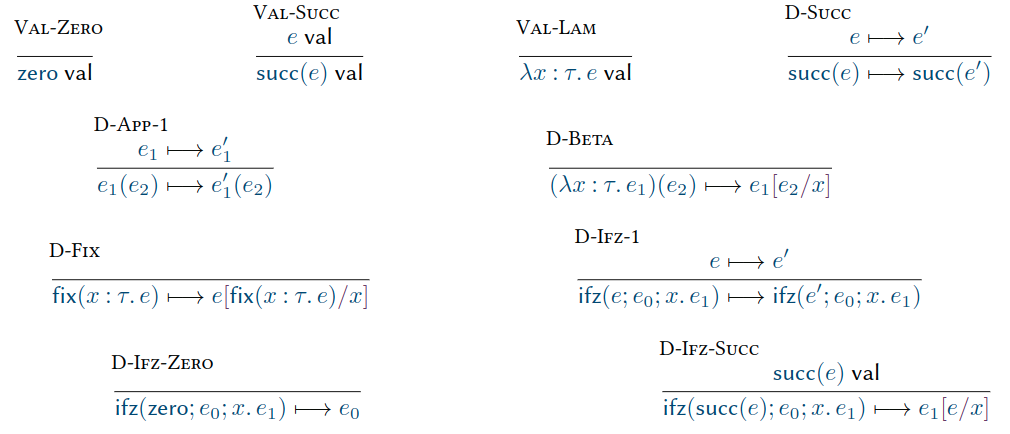
\includegraphics[width=\textwidth]{pics/dynamic-pcf.png}

\newpage
\section{Call by Value/Name}
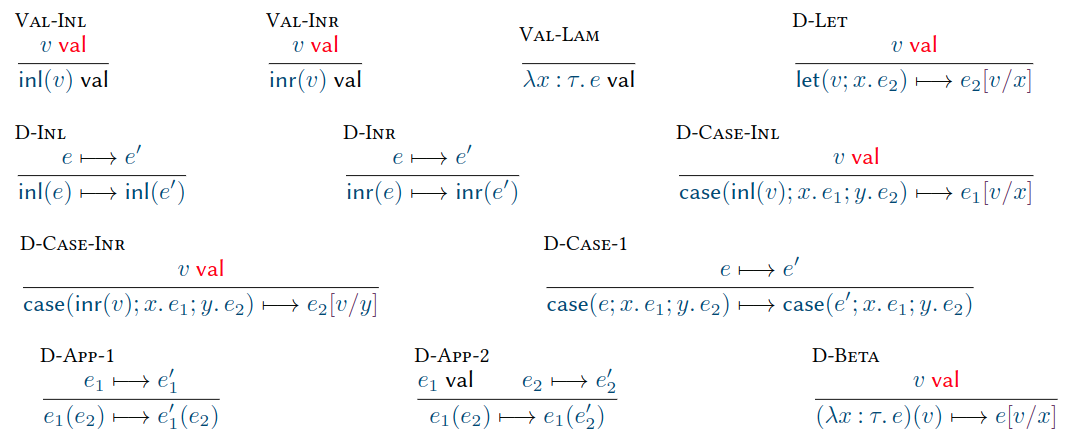
\includegraphics[width=\textwidth]{pics/cbv.png}

\subsection{Process order}
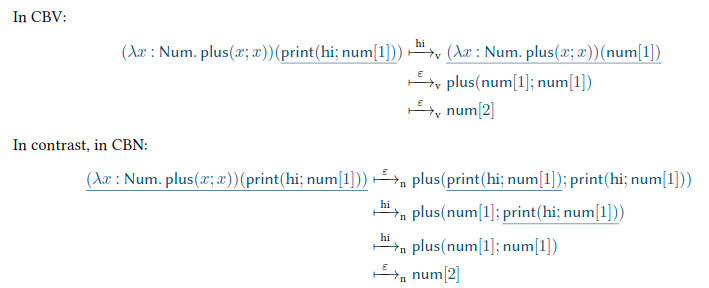
\includegraphics[width=\textwidth]{pics/cbnvscbv.png}

\newpage
\section{Store}
\subsection{Syntax}
\begin{center}
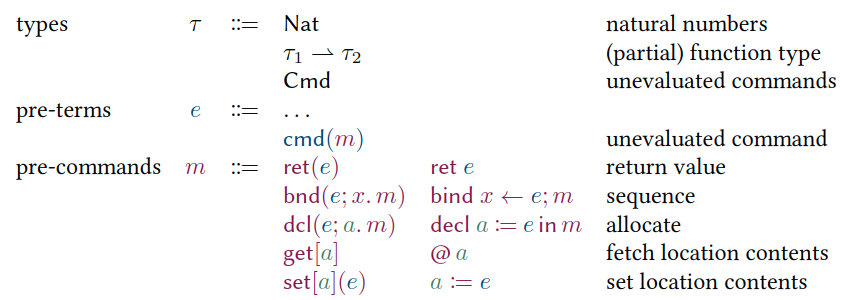
\includegraphics[width=\textwidth/3*2]{pics/syntax-store.png}
\end{center}
\subsection{Statics}
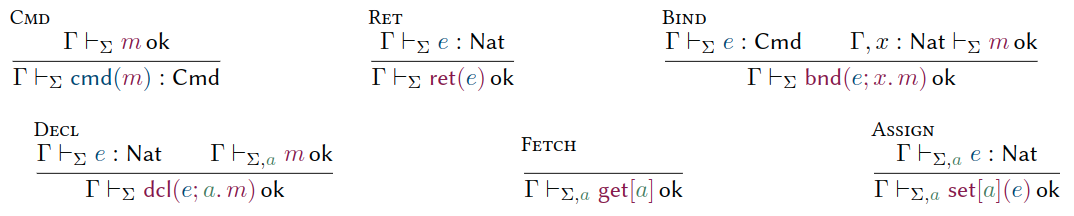
\includegraphics[width=\textwidth]{pics/static-store.png}
\subsection{Transitions}
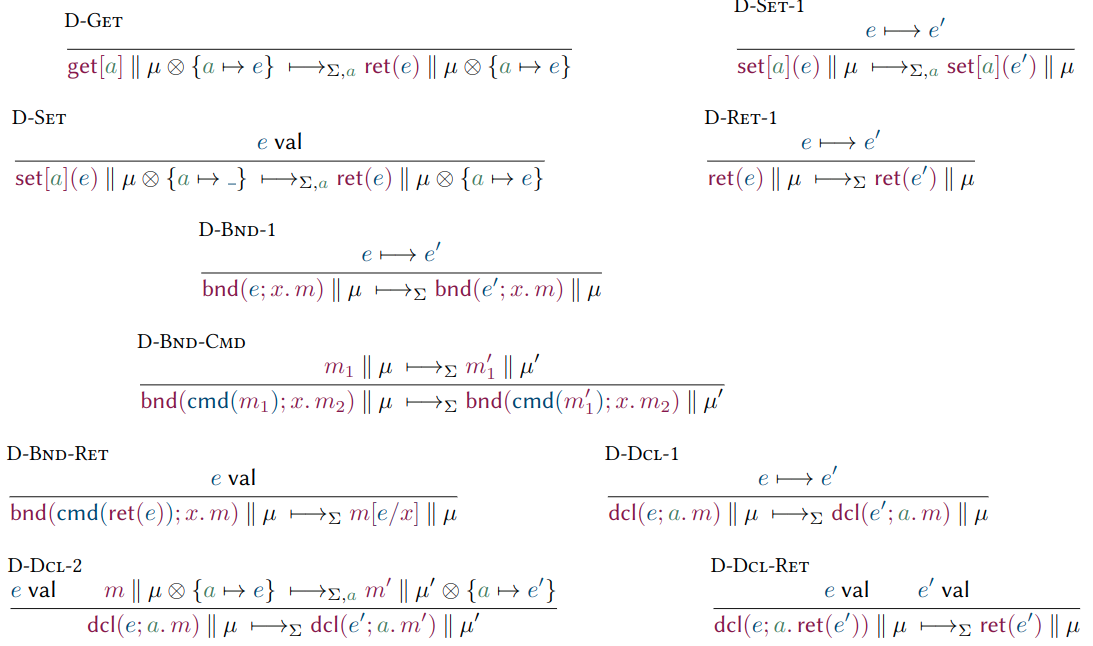
\includegraphics[width=\textwidth]{pics/dynamic-store.png}




\end{document}